An SQL database is used for the backend database. 

The following information is required:
{\it TO BE REVIEWED}
\begin{itemize}
\item Super User name or egroup
\item Roles
\item Map of user names or egroups to roles
\item list of resource pools
\item meta data of resource pools
\end{itemize}

{\it ADD FEEDBACK LOOP}
The database holds all dynamic information. Static configuration data goes into the configuration files, see there. 
Certain information like the meta data of resource pools may change during the lifetime of the product. The database schema is made in such a way that it is easy to add or remove features which were not there at the beginning to the schema without having to perform complicated and slow database operations. 

\begin{figure}
\begin{center}
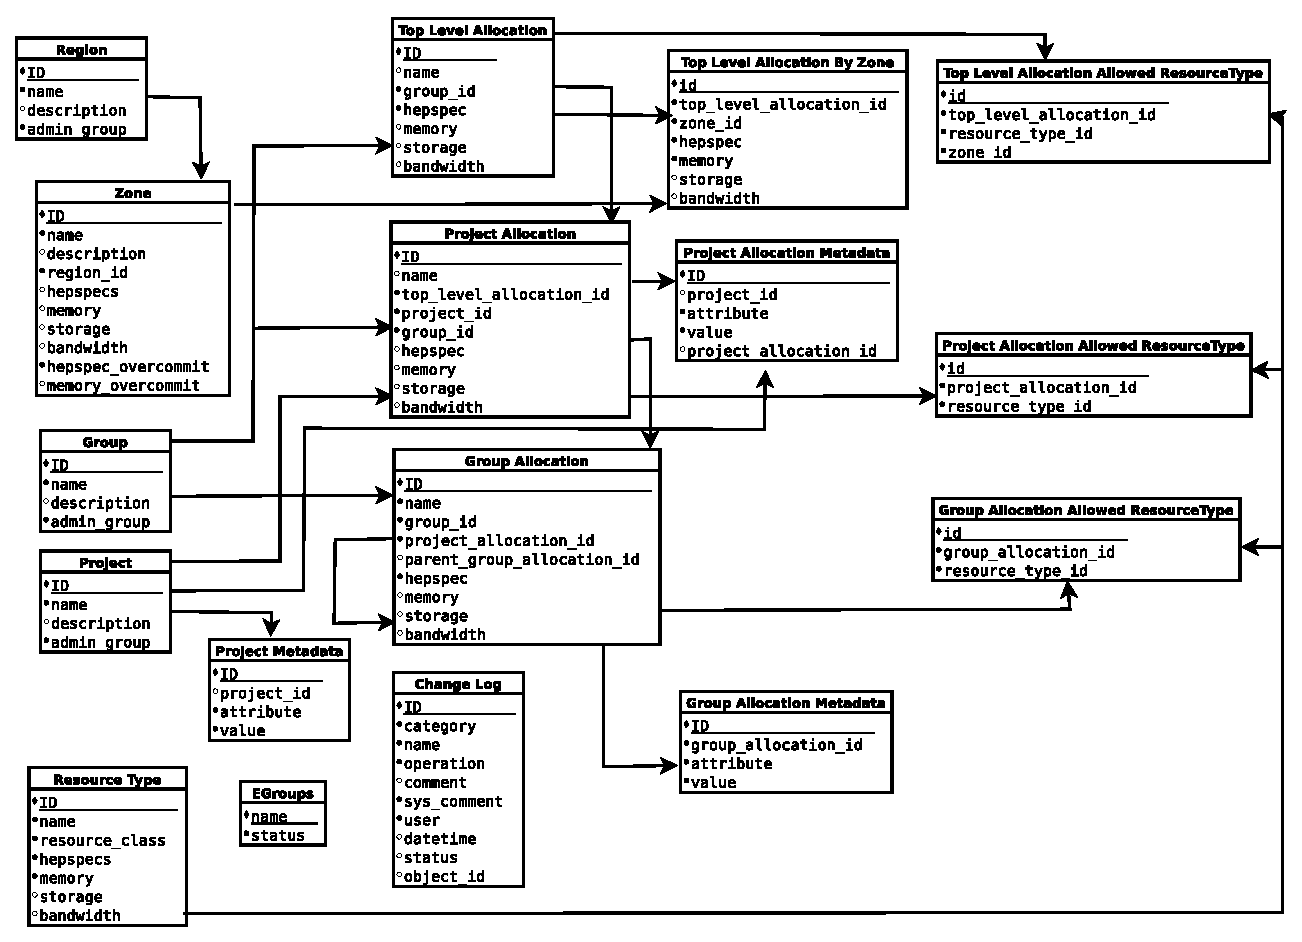
\includegraphics[width=\textwidth]{cloudman_db.eps}
\caption{\label{ddb_schema_new} Cloudman database schema, Aldebaran Release.}
\end{center}
\end{figure}

The figure ~\ref{ddb_schema_new} shows the final database schema for the Aldebaran release of CloudMan.


The description of resources is kept in the database as well. This way, it is easy to define new valid resource attributes directly via the web interface. Updating this table is reserved to the resource manager role who owns all privileges. 

Resources and groups are matched at the top level by the resource manager in the process of filling in the allocations. Allocations are done in terms of CPU, disk and memory for each resource available. 
The resource manager approves requests for the allocations. Only approved allocations will be exported, 
and used by the back-ends.

At the lower levels, the managers do allocations out of the quota which have been allocated to them by an upper instance. 



